\documentclass{article}
\usepackage[utf8]{inputenc}
\usepackage[ukrainian]{babel}
\usepackage{graphicx}
\usepackage{hyperref}
\usepackage{tabularx}
\usepackage{booktabs}
\usepackage{xcolor}
\usepackage{subcaption}
\usepackage{float}

\title{Модель пухлини на основі клітинного автомата}
\date{}

\begin{document}

\maketitle

\tableofcontents

\newpage

\section{Вступ}
Короткий опис мети проєкту, його значущості та обраного підходу моделювання (стохастичний клітинний автомат).

\section{Теоретичні основи}
\subsection{Клітинні автомати в моделюванні раку}
Пояснення, чому клітинні автомати підходять для просторово-часового моделювання пухлин.

\subsection{Ієрархія клітин пухлини}
Опис біологічної структури клітин:

\maketitle

\section*{1. \textbf{Cell (Базова клітина)}}
Базовий клас для всіх типів клітин.

\begin{itemize}
    \item Координати: $x$, $y$
    \item Таймер поділу: \texttt{time\_since\_division}
    \item Кількість доступних поділів: \texttt{divisions\_left}
    \item Час циклу клітини: \texttt{cct} = 24 годин
    \item Стан життя: \texttt{is\_alive}
\end{itemize}

\noindent \textbf{Методи:}
\begin{itemize}
    \item \texttt{can\_divide()}
    \item \texttt{reset\_timer()}
    \item \texttt{update\_timer(dt)}
    \item \texttt{die()}
    \item \texttt{migrate(free\_neighbors)}
\end{itemize}

\section*{2. \textbf{EmptyCell (Порожня клітинка)}}
\begin{itemize}
    \item Просто ``місце'', де немає клітини.
    \item \texttt{is\_alive = False}
    \item Не ділиться.
\end{itemize}

\section*{3. \textbf{NecroticCell (Некротична клітина)}}
\begin{itemize}
    \item Мертва клітина, яка раніше була живою, але вже не функціонує.
    \item \texttt{is\_alive = False}
    \item Не ділиться.
\end{itemize}

\section*{4. \textbf{RegularTumorCell (Звичайна пухлинна клітина)}}
\begin{itemize}
    \item Має обмежену кількість поділів.
    \item \texttt{divisions\_left} зменшується з кожним поділом.
    \item Якщо \texttt{divisions\_left} $\leq 2$, перетворюється на \texttt{NecroticCell} при наступному поділі.
    \item Метод \texttt{divide()} створює нову \texttt{RegularTumorCell} з \texttt{divisions\_left - 1}.
\end{itemize}

\section*{5. \textbf{StemTumorCell (Стовбурова пухлинна клітина)}}
\begin{itemize}
    \item Необмежена здатність до поділу: \texttt{divisions\_left = \(\infty\)}.
    \item Завжди ділиться у \texttt{RegularTumorCell}.
    \item Символізує агресивну форму пухлини.
\end{itemize}

\section*{6. \textbf{TrueStemCell (Істинна стовбурова клітина)}}
\begin{itemize}
    \item Найбільш ``основна'' стовбурова клітина.
    \item Може створювати:
    \begin{itemize}
        \item ще одну \texttt{TrueStemCell} з імовірністю $\rho$
        \item або \texttt{StemTumorCell} з імовірністю $1 - \rho$
    \end{itemize}
    \item Має потенціал підтримувати як нормальну, так і пухлинну популяцію.
\end{itemize}

\section*{7. \textbf{ImmuneCell (Імунна клітина)}}
\begin{itemize}
    \item Може атакувати пухлинні клітини.
    \item Має такі характеристики:
    \begin{itemize}
        \item \textbf{Тривалість життя}: \texttt{lifespan}, напр., 72 год.
        \item \textbf{Ймовірність вбивства клітини}: \texttt{kill\_probability}, напр., 0.3
        \item \textbf{Рівень активації}: \texttt{activation\_level} — підсилює здатність убивати
        \item \textbf{Кількість поділів}: обмежена, напр., 3
        \item Помирає при досягненні \texttt{age} $\geq$ \texttt{lifespan}
    \end{itemize}
\end{itemize}

\subsection{Динаміка росту пухлини}
Основні події життєвого циклу клітин:
\begin{itemize}
    \item Поділ
    \item Міграція
    \item Смерть
    \item Вибір шляху диференціації
\end{itemize}

\subsection{Взаємодія з імунною системою}
Механізми імунної відповіді:
\begin{itemize}
    \item Активація
    \item Знищення клітин пухлини
    \item Міграція та поділ імунних клітин
    \item Тривалість життя імунних клітин
\end{itemize}

\section{Реалізація}
\subsection{Архітектура моделі}
\begin{itemize}
    \item Решітка (Grid)
    \item Клас клітин (Cell)
    \item Симулятор (TumorSimulation)
\end{itemize}

\subsection{Основні параметри}

У цьому розділі коротко описуються ключові параметри, що використовуються в моделі.

\subsection{Алгоритм симуляції}
Покроковий опис:
\begin{enumerate}
    \item Оновлення клітин пухлини
    \item Оновлення імунних клітин (якщо увімкнено)
    \item Збір статистики
\end{enumerate}

\section{Результати симуляції}

\subsection{Візуалізація та колірна схема}

Для інтерпретації результатів симуляції застосовується наступна колірна схема клітин:

\begin{itemize}
    \item \textcolor{blue}{\rule{1em}{1em}} Імунні клітини (Immune cells)
    \item \textcolor{orange}{\rule{1em}{1em}} Некротичні клітини (Necrotic cells)
    \item \textcolor{gray}{\rule{1em}{1em}} Порожні клітини (вільний простір)
    \item \textcolor{yellow}{\rule{1em}{1em}} Істинні стовбурові клітини (True Stem Cells)
    \item \textcolor{green}{\rule{1em}{1em}} Стовбурові пухлинні клітини (Stem Tumor Cells)
    \item \textcolor{red}{\rule{1em}{1em}} Звичайні пухлинні клітини (Regular Tumor Cells), з градацією відтінків залежно від кількості поділів
\end{itemize}

\subsection{Динаміка росту пухлини без імунної відповіді}
На рисунках нижче показано просторову динаміку росту пухлини без впливу імунної системи. Видно поступове збільшення маси пухлини та утворення некротичного ядра.

\begin{figure}[H]
    \centering
    \begin{subfigure}[t]{0.32\linewidth}
        \centering
        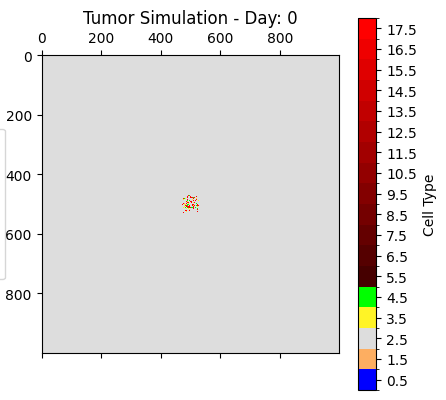
\includegraphics[width=\linewidth]{tumor_simulation_stats/tumor_day_0.png}
        \caption{День 0}
        \label{fig:tumor-day-0-no-immune}
    \end{subfigure}
    \hfill
    \begin{subfigure}[t]{0.32\linewidth}
        \centering
        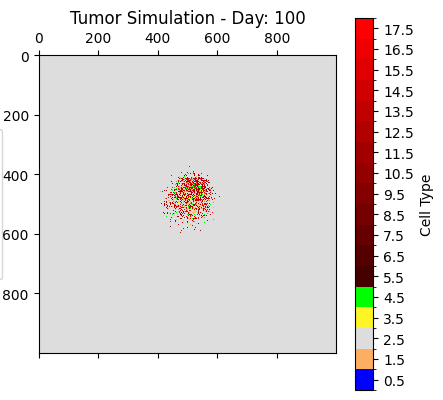
\includegraphics[width=\linewidth]{tumor_simulation_stats/tumor_day_100.png}
        \caption{День 100}
        \label{fig:tumor-day-100-no-immune}
    \end{subfigure}
    \hfill
    \begin{subfigure}[t]{0.32\linewidth}
        \centering
        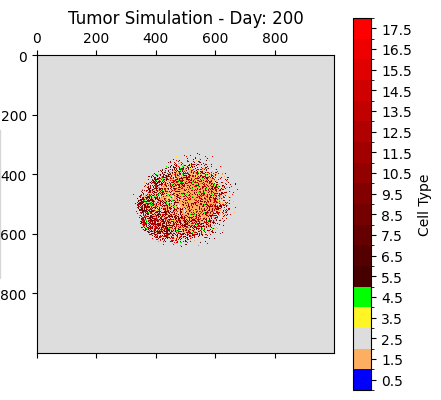
\includegraphics[width=\linewidth]{tumor_simulation_stats/tumor_day_200.png}
        \caption{День 200}
        \label{fig:tumor-day-200-no-immune}
    \end{subfigure}
    \label{fig:tumor-evolution-no-immune}
\end{figure}

\subsection{Динаміка росту пухлини з імунною відповіддю}
Далі представлено вплив імунної системи на динаміку пухлини. Імунні клітини поступово проникають у пухлину, взаємодіють з нею, зменшуючи кількість активних пухлинних клітин.

\begin{figure}[H]
    \centering
    \begin{subfigure}[t]{0.32\linewidth}
        \centering
        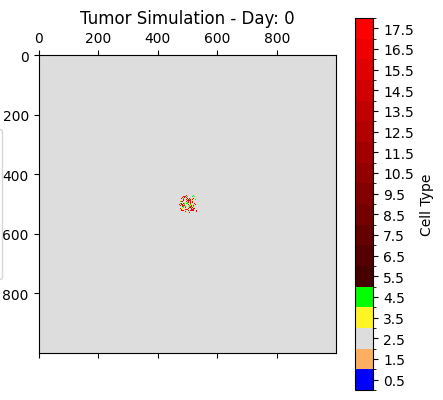
\includegraphics[width=\linewidth]{tumor_immune_simulation_stats/tumor_immune_day_0.png}
        \caption{День 0}
        \label{fig:tumor-day-0-immune}
    \end{subfigure}
    \hfill
    \begin{subfigure}[t]{0.32\linewidth}
        \centering
        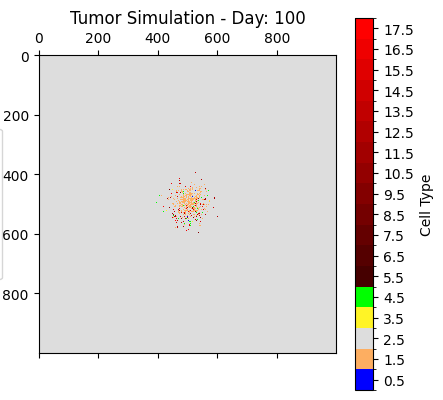
\includegraphics[width=\linewidth]{tumor_immune_simulation_stats/tumor_immune_day_100.png}
        \caption{День 100}
        \label{fig:tumor-day-100-immune}
    \end{subfigure}
    \hfill
    \begin{subfigure}[t]{0.32\linewidth}
        \centering
        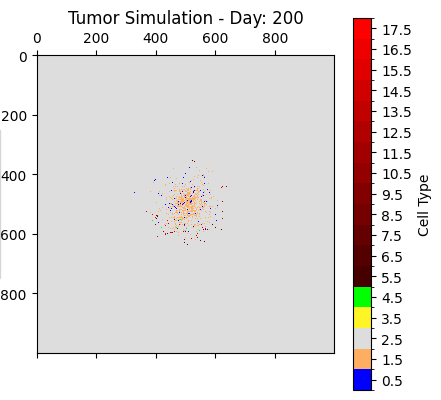
\includegraphics[width=\linewidth]{tumor_immune_simulation_stats/tumor_immune_day_200.png}
        \caption{День 200}
        \label{fig:tumor-day-200-immune}
    \end{subfigure}
    \label{fig:tumor-evolution-immune}
\end{figure}

\subsection{Графіки популяцій клітин}
На графіках показано кількісні зміни популяцій клітин протягом симуляції. Це дозволяє оцінити темпи росту пухлини, активність імунної системи, а також частку некротичних клітин.

\begin{figure}[H]
    \centering
    \begin{subfigure}[t]{0.75\linewidth}
        \centering
        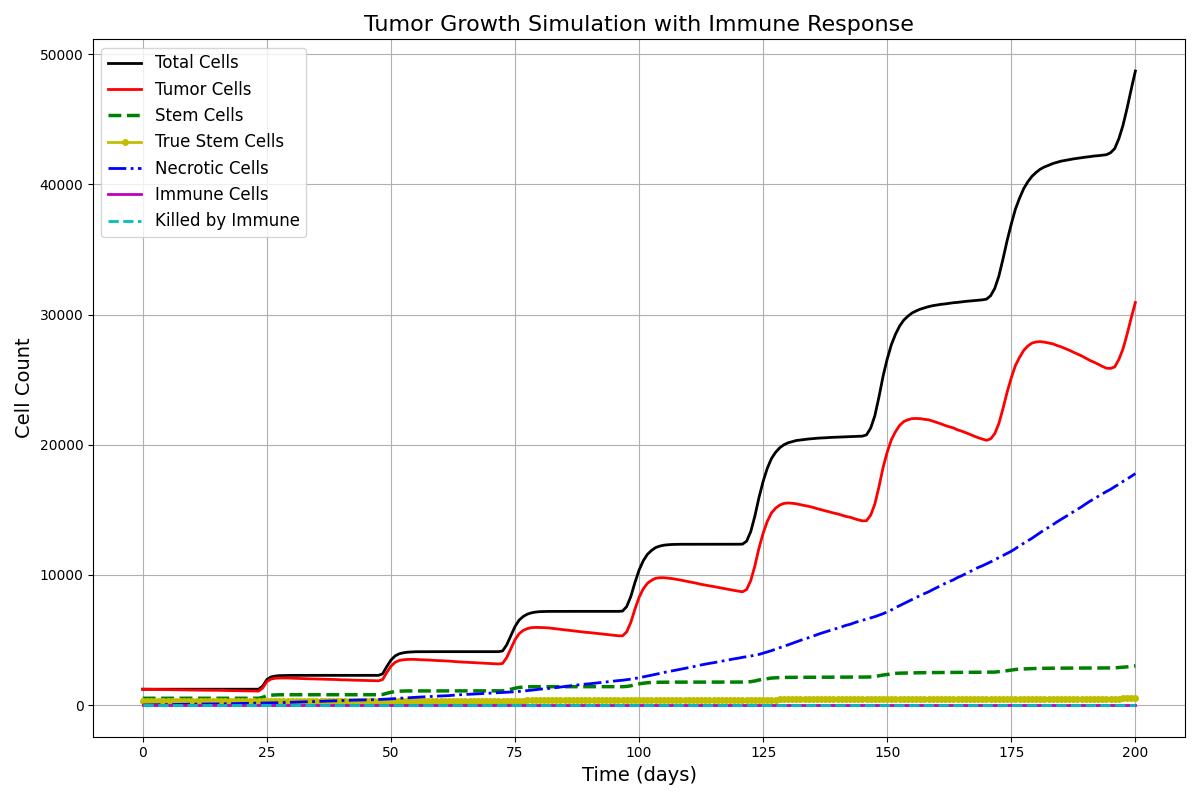
\includegraphics[width=\linewidth]{tumor_simulation_stats/tumor_stats.png}
        \caption{Динаміка популяцій клітин без імунної відповіді}
        \label{fig:tumor-stats-no-immune}
    \end{subfigure}
    
    \begin{subfigure}[t]{0.75\linewidth}
        \centering
        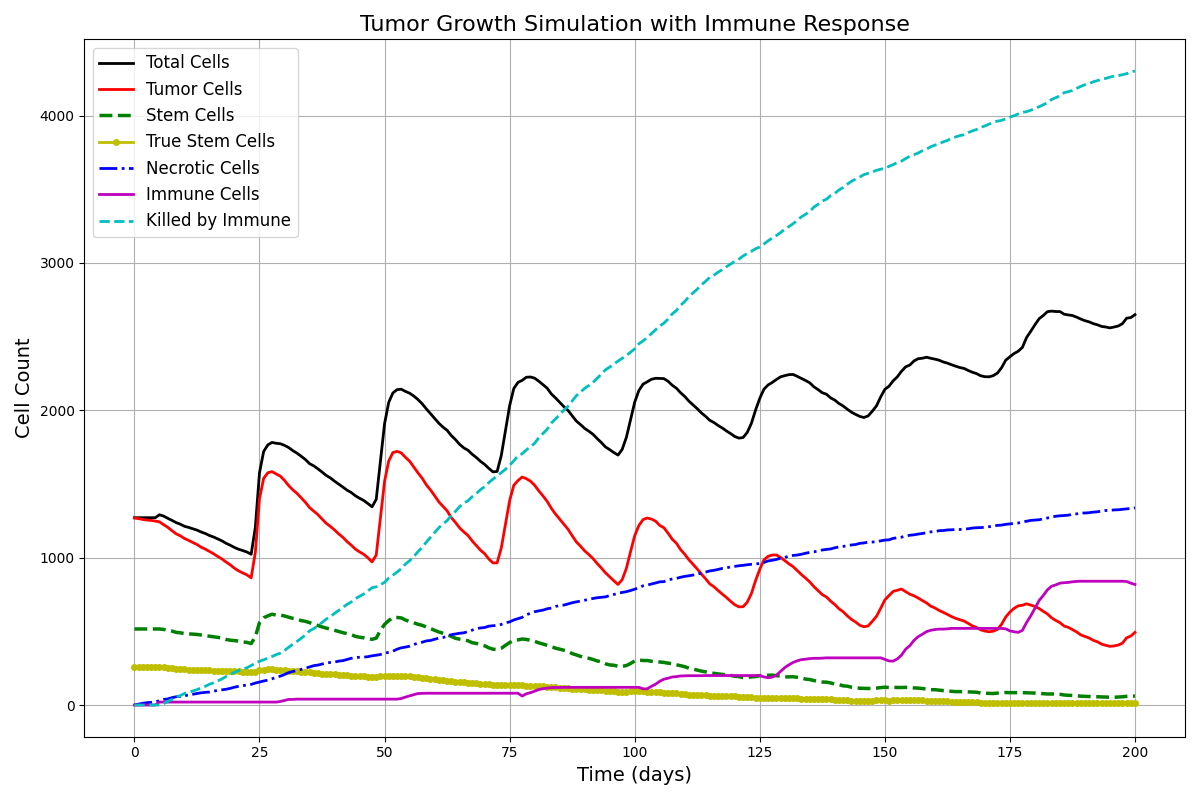
\includegraphics[width=\linewidth]{tumor_immune_simulation_stats/tumor_immune_stats.png}
        \caption{Динаміка популяцій клітин з імунною відповіддю}
        \label{fig:tumor-stats-immune}
    \end{subfigure}
    \label{fig:stats-comparison}
\end{figure}

\section{Учасники проєкту}
\begin{itemize}
    \item Ярина Печененко – логіка клітин
    \item Іван Зарицький – візуалізація, CLI
    \item Михайло Рихальський – структура решітки, просторова логіка
    \item Роман Прохоров – движок симуляції
\end{itemize}

\section{Ментор}
Максим Жук

\end{document}